\documentclass{../res/univ-projet}

%Import des packages utilisés pour le document
\usepackage[utf8x]{inputenc}
\usepackage[francais]{babel}
\usepackage[T1]{fontenc}

%Redéfinition des marges
\addtolength{\topmargin}{-1cm}
\addtolength{\textheight}{1cm}
\addtolength{\headsep}{0.8cm}
\addtolength{\footskip}{-0.2cm}

%Variables
\logo{../res/logo_univ.png}
\title{Document d'architecture du logiciel}
\author{Matthieu \bsc{Fin}, Guillaume \bsc{Leroy}}
\projet{GPG}
\projdesc{Interface Graphique GPG}
\filiere{M1SSI - Conduite de Projet}
\version{0.1}
\relecteur{}
\signataire{Magali \bsc{Bardet}}
\date{\today}


\histentry{0.1}{23/11/2014}{Version initiale.}

% definition d'un bleu un peu moins criard que celui par defaut ...
\definecolor{blue_saphir}{rgb}{0,.19,.71}

% Commande permettant de créer un tableau entrées / sortie / pré-post conditions pour les méthodes
\newcommand{\methode}[6]{
  \begin{tabular}{|>{\centering}p{2.5cm}|>{\centering}p{7cm}|}
    \hline
    \color{white}\cellcolor{blue_saphir}\bfseries{Nom}&
    #1 \cr
    \hline
    \color{white}\cellcolor{blue_saphir}\bfseries{Entrée}&
    #2 \cr
    \hline
    \color{white}\cellcolor{blue_saphir}\bfseries{Préconditions}&
    #3 \cr
    \hline
    \color{white}\cellcolor{blue_saphir}\bfseries{Sortie}&
    #4 \cr
    \hline
    \color{white}\cellcolor{blue_saphir}\bfseries{Postconditions}&
    #5 \cr
    \hline
    \color{white}\cellcolor{blue_saphir}\bfseries{Description}&
    #6 \cr
    \hline
  \end{tabular}\\
}

% -- Début du document -- %
\begin{document}

%Page de garde
\maketitle
\newpage
%La table des matières
\tableofcontents
\newpage

\section{Objet}
  \methode{Test}{Paramètres}{Paramètres != NULL}{Miaou}{Miaou = 6}{Ceci est un test}
  Ce document permet d'établir une vue globale de l'architecture logicielle envisagée pour la conception d'une interface graphique reposant sur le logiciel GnuPG de façon à simpliciter son utilisation pour un utilisateur débutant mais toutefois en laissant apparaitre les fonctionnalités avancées pour un utilisateur expérimenté. Il décrit comment concevoir cette interface pour répondre aux spécifications du client ainsi qu'une conception détaillée des différents modules nécessaires à son bon fonctionnement. 

\section{Documents applicables et de référence}
  \begin{itemize}
    \item La spécification technique des besoins
  \end{itemize}

\section{Terminologie et sigles utilisés}
  \subsection{Acronymes}
    \begin{itemize}
      \item GNOME GNU Network Object Model Environment
      \item GNU GNU's Not UNIX
      \item IETF Internet Engineering Task Force
      \item KDE K Desktop Environment
      \item MVC Model View Controller
      \item PGP Pretty Good Privacy
      \item RFC Request For Comments
    \end{itemize}

  \subsection{Glossaire}
    \begin{itemize}
      \item C++\\
        Langage de programmation compilé.
      \item Environement de bureau\\
        Ensemble de programmes qui permettent de manipuler le système à travers une interface graphique.
      \item MVC\\
        Patron de conception répondant aux besoins des applications intéractives en séparant les problèmatiques en trois parties :
        \begin{itemize}
          \item Le modèle\\
            Il représente les données manipulées par l'application et est responsable de leur intégrité.
          \item La vue\\
            Ce avec quoi l'utilisateur interagit. Sa fonction principale est d'afficher les données envoyées par le modèle.
          \item Le controller\\
            Il traite les évenements et met à jour la vue ou le modèle selon l'action effectuée.
        \end{itemize}
      \item Qt\\
        Interface de programmation orientée objet développée en C++ permettant la conception simple d'interface graphique compatible GNU Linux / Windows / Mac OS X.
    \end{itemize}

\section{Configuration requise}
  \subsection{Système d'exploitation}
    GNU Linux
  \subsection{Logiciels}
    Environement de bureau KDE (v4.0 ou ultérieure) ou GNOME (v3.0 ou ultérieure)\\
    GnuPG (v1.4 ou ultérieure)
  \subsection{Matériel}
    Aucune configuration minimale n'est demandée.

\section{Architecture statique}
  \subsection{Structure} % (fold)
    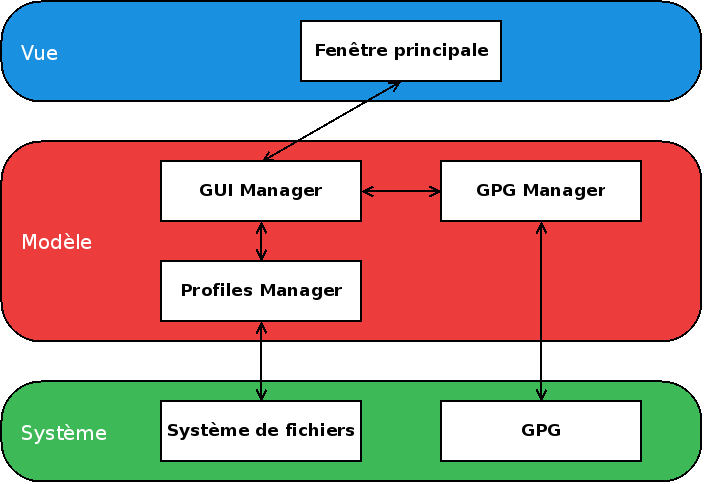
\includegraphics[scale=0.5]{graphics/diagramme_archi.png}
  \subsection{Description du constituant "X"} % (fold)
    \textcolor{blue}{
      TODO : \\
      {\begin{itemize}
        \item Rôle.
        \item Propriétés et attributs de caractérisation.
        \item Services offert (interfaces)
        \item Dépendances avec d'autres constituants (service utilisés,
        composants "sur étagère" utilisés)
        \item Langage de programmation
        \item Procédé de développement (techniques, méthodes et/ou outils)
        \item Taille et complexité.
      \end{itemize}}
    }
  % subsection Description du constituant "X" (end)
  \subsection{Justification techniques} % (fold)
    \textcolor{blue}{
      TODO : \\
      Fournir une rapide justification des choix technique originaux.
    }
  % subsection justification_techniques (end)
\section{Fonctionnement dynamique} % (fold)
\label{sec:fonctionnement_dynamique}

  \textcolor{blue}{
    TODO : \\
    Pour les principaux scénarii identifiés dans la spécification technique de besoin.
    \begin{itemize}
      \item Liste des composants mis en jeu.
      \item Description du processus de mise en oeuvre sous la forme d'une
      séquence d'appels aux services offerts par les différents composants et en faisant
      clairement apparaître
      \begin{itemize}
        \item la logique et le flux des événements traités
        \item les interactions du logiciels avec les acteurs
        \item les interactions entre les composants au travers de leurs interfaces
      \end{itemize}
    \end{itemize}
  }

% section fonctionnement_dynamique (end)
\section{Traçabilité} % (fold)
\label{sec:tra_abilit_}

  \textcolor{blue}{
    TODO : \\
    Récapitulatif des liens de dépendance entre les constituants du logiciel et les exigences de
    la STB (par exemple sous forme de tableau).
  }

% section tra_abilit_ (end)
\end{document}

